% SPDX-License-Identifier: CC-BY-SA-4.0
%
% Copyright (c) 2021 Philipp Le
%
% Except where otherwise noted, this work is licensed under a
% Creative Commons Attribution-ShareAlike 4.0 License.
%
% Please find the full copy of the licence at:
% https://creativecommons.org/licenses/by-sa/4.0/legalcode

\chapter{Information and Coding Theory}

\begin{refsection}

Information exchange through a transmission channel is always subject to noise. Spread spectrum techniques can be used to harden the transmission against noise up a certain extent. However, noise and its disturbance on the information transmission cannot be completely avoided. ``Hardening against noise'' actually means: Reducing the probability of getting a wrongly decoded signal in the receiver.

As everything related to noise, statistics and probability are central terms. There is always a non-zero probability of modulating an erroneous signal. The probability increases as the \ac{SNR} decreases. A measure for the errors after signal demodulation is the \textbf{\acf{BER}} \index{bit error rate}, when binary symbols (bits) are transmitted. It is the ratio of the number of erroneously received bits $N_{err}$ divided by the number of totally transmitted bits $N_{tot}$.

\begin{equation}
	\mathrm{BER} = \frac{N_{err}}{N_{tot}}
\end{equation}
\nomenclature[B]{$mathrm{BER}$}{Bit error rate}%

Even with a good \ac{SNR}, there is a small probability for receiving wrong bits and the \ac{BER} is greater than zero, even if close to zero. But, already one false bit may corrupt the communication, for example if a complex protocol is used in a higher layer of the \ac{OSI} stack.

In the chapter, techniques to deal with corrupt symbols will be discussed. By adding some redundancy, falsely demodulated symbols can be detected and even corrected. This ensures a reliable communication in the presence of noise. Even harsh condition with low \ac{SNR} can be mastered. Nowadays, the electromagnetic spectrum is used heavily by a huge number of services. Their signals may cause disturbances to each other (noise). Without error correction methods, it would be difficult to reliably communicate.

The basis for these symbol recovery techniques is proper \index{coding} \emph{coding}. \index{information and coding theory} \textbf{Information and coding theory} is the study of mathematical methods to describe information and their processing. Here, information are not considered as signals as in the chapters before -- information is now a discrete entity, which is the subject of mathematical analysis.

The applications of \emph{information and coding theory} are:
\begin{itemize}
	\item \textbf{Source coding}: Detecting and removing unnecessary redundancy in a stream of symbols. This also known as \emph{compression}.
	\item \textbf{Channel coding}: Adding systematically redundancy to a stream of symbols, in order to be able to detect and correct transmission errors in the receiver.
	\item \textbf{Cryptography}: Concealing the contents of the transmission to provide confidentiality.
	\item \textbf{Line coding}: Bringing the information into a representation, so that the transmission channel can transfer the information. (Not all signal representations of information can be transmitted equally, because they have different physical properties (bandwidth, etc.).) Actually, the line coding operates in the baseband. The line-coded baseband signal is than given to a mixer, which then produces the \ac{RF} signal for transmission over the channel.
\end{itemize}

% TODO: Maybe some line coding too
This chapter concerns with \emph{source coding} and \emph{channel coding}. They are the last missing part in our signal and information processing chain in a digital communication system.
\begin{itemize}
	\item Modulation brings the information onto a carrier which can be transmitted through a transmission channel.
	\item Spread spectrum and multiple access enabled sharing the transmission channel with different users.
	\item Source coding reduces the amount of data which must be transmitted (compression) and thereby improves the performance (data rate).
	\item Channel coding hardens the signal transmission against noise and disturbances. Erroneous symbols can be detected and corrected using mathematical methods.
\end{itemize}

% TODO: Figure showing the processing chain

It is important to note, that even channel coding cannot push the error probability or \ac{BER} down to exactly zero. A probability of decoding symbols wrongly is still there. However, channel coding significantly reduces this probability. The probability is so low, that it almost does not matter is reality. This is the criterion for a reliable communication.

\section{Information Model}

Information considered in a digital communication system is value-discrete. The information is represented by a set of symbols $x_i$ which is the \index{source alphabet} \emph{source alphabet} $\Omega$. Considering there are $M$ discrete symbols, the source alphabet is:

\begin{equation}
	\Omega = \bigcup\limits_{i = 1}^{M} x_i = \left\{x_1, x_2, \ldots, x_M\right\}
\end{equation}
\nomenclature[U]{$\bigcup\limits_{i = 1}^{M}$}{Union of sets}

All information originates from a source -- the information source in the Shannon-Weaver model. Here, it is called a \index{discrete information source} \emph{discrete information source}. The discrete information sources emits a series of discrete information (symbols) from the source alphabet $\Omega$. The series of symbols is then processed by further parts of the communication system -- coding, spreading, modulation, etc.

In this chapter, the actual content of the information is not important. The real interpretation of the symbols is a matter of the user of the communication system or higher layers in the \ac{OSI} stack, which is modelled as the discrete information source. Here, the information is just considered as symbols which are emitted by an abstract discrete information source.

\subsection{Memoryless Information Source}

A \index{message} \textbf{message} is a series of symbols out of the alphabet $\Omega$ which is emitted by a discrete information source. The message $\vec{m}$ has a length of $N_m$.
\begin{equation}
	\vec{m} = \left[x[0], x[1], \ldots, x[N_m-1]\right]
\end{equation}
$x[n] \in \Omega$ is a symbol of the source alphabet $\Omega$. $n$ is the index of the symbol in the message.

$x[n]$ can be any symbol\footnote{In the literature, \textbf{event} is used as a synonym, too. Here, we stick to \emph{symbol} to make the relationship to the symbols used for modulation and spreading clear.} $x_i \in \Omega$ out of the source alphabet. Now, the discrete information source is considered to be a black-box. It emits a series of symbols. But from the outside, a observer has no knowledge about the internals (like a algorithm which generates the symbols). So the symbol emission is random. The discrete information source is a random process. The emitted symbol $x[n]$ is a random variable.

In addition to the randomness of symbol emission, it is assumed that the source has no memory. That is, the emission of a symbol $x[n]$ does not depend on the past symbols $x[0], \ldots, x[n-1]$. So all samples (i.e. symbols) taken from the discrete information source are independent from each other. As a consequence, the discrete information source does not have an internal memory, which stores past symbols which upcoming symbols rely on. The source is a \index{discrete memoryless source} \textbf{discrete memoryless source}.

\begin{excursus}{Sources with memory}
	Of course, there are sources with a memory. Here, a emitted symbol depends on past symbols.
	
	An example is written English language. The symbols are the letters. The source alphabet comprises 26 letters. A random sequence of letters like ``qwubrfasdfnas'' does not make any sense. The letters in the sequence always depend on other letters to form words. Some letters like ``q'' furthermore only exist together with other letters (``qu'').
\end{excursus}

Each symbol $x_i$ has a certain probability $p_i$ of being emitted by the discrete information source. The occurence probabilities of all symbols must sum to $1$.

\begin{equation}
	\sum\limits_{i=1}^{M} p_i \stackrel{!}{=} 1
	\label{eq:ch08:dms_prob_sum}
\end{equation}

So a message $\vec{m}$ with a length of $N_m$ contains the symbol $x_i \in \Omega$ in average $N_m p_i$ times.

\begin{proof}{}
	The total length of the message $\vec{m}$ is the sum of the average number of occurences $N_m p_i$ of all $M$ symbols.
	\begin{equation}
		\begin{split}
			\dim \vec{m} &= \sum\limits_{i=1}^{M} N_m p_i \\
			 &= N_m \cdot \underbrace{\sum\limits_{i=1}^{M} p_i}_{= 1, \, \text{because of \eqref{eq:ch08:dms_prob_sum}}} \\
			 &= N_m
		\end{split}
	\end{equation}
	So the length of the message $\vec{m}$ is indeed $N_m$.
\end{proof}

A message where all symbols $x_i$ occur exactly $N_m p_i$ times is called a \textbf{typical sequence}. The position of the symbols $x_i$ are not fixed in the message. So, there are $N_{TS}$ possible combinations of typical sequences. The probability that a typical sequence of a certain combination is emitted is $P_{TS}$.
\begin{equation}
	P_{TS} = \prod\limits_{i = 1}^{M} p_i^{N_m p_i} = p_1^{N_m p_1} \cdot p_2^{N_m p_2} \cdot \ldots \cdot p_M^{N_m p_M}
	\label{eq:ch08:typseq_prob}
\end{equation}%
\nomenclature[Pts]{$P_{TS}$}{Probability that a typical sequence of a certain combination is emitted}%
According to Shannon, only typical sequences shall be considered, because all other sequences are very unlike to occur.
\begin{equation}
	\begin{split}
		N_{TS} \cdot P_{TS} &\stackrel{!}{=} 1 \\
		N_{TS} &= \frac{1}{P_{TS}} \\
		 &= \frac{1}{\prod\limits_{i = 1}^{M} p_i^{N_m p_i}}
	\end{split}
\end{equation}

\subsection{Information Content}

At this point, a \emph{discrete memoryless source} emits a sequence of symbols. The sequence of symbols -- the \emph{message} -- carries the \index{information} \textbf{information}. So the complete information is distributed over the symbols in the sequence.

Now considering each symbol $x_i \in \Omega$ independently, what is the contribution of that symbol $x_i$ to the information? A measure is the \index{information content} \textbf{information content} $\mathrm{I}(x_i)$ of the symbol $x_i \in \Omega$. \nomenclature[I]{$\mathrm{I}(x_i)$}{Information content of the symbol $x_i \in \Omega$}

The information content only depends on the probability of the symbol $p_i$, i.e. $\mathrm{I}(x_i)$ is a function of $p_i$.
\begin{equation}
	\mathrm{I}(x_i) = f(p_i)
\end{equation}
The function $f(\cdot)$ needs to be determined.

$\mathrm{I}(x_i)$ has some constraints.
\begin{itemize}
	\item If $p_i = 1$, then $\mathrm{I}(x_i) = 0$. $p_i = 1$ means that the source emits $x_i$ only. This makes the discrete memoryless source predictable. As a consequence, the message generated by this source does not contain any information -- the information content $\mathrm{I}(x_i)$ is zero. Remember that information leads to an increased knowledge in the receiver (Shannon-Weaver model in Chapter 1). A receiver cannot gain any knowledge from a predictable source, because it already has the knowledge ``there is only $x_i$''.
	\item Consequently, if $p_i < 1$, then $\mathrm{I}(x_i) > 0$.
\end{itemize}
Furthermore, $\mathrm{I}(x_i)$ must be non-negative.

\begin{example}{}
	The information content is some kind of measure of the worth a symbol. The higher the information content is, the more knowledge is gained in the receiver.
	
	Let's illustrate the worth: The information content $\mathrm{I}(x_i)$ is a function of the probability $p_i$ of the event (symbol) $x_i$.
	\begin{itemize}
		\item A very probable event is that a good friend is visiting you regularly for hanging-out. So you won't put much expense in tidy up your apartment.
		\item A less probable event is a visit by your grandparents. You want to make a good impression and clean every corner in your apartment. The expense is much higher.
	\end{itemize}
\end{example}

Let's define a event $C$ generated by the source. $C$ is a message composed of the symbols $x_1$ and $x_2$. So, $C$ is the intersection of $x_1$ and $x_2$.
\begin{equation}
	C = x_1 \cap x_2
\end{equation}

Because the symbols $x_1$ and $x_2$ are independent in a discrete memoryless source, the probability $\mathrm{P}(C)$ that the event $C$ occurs is:
\begin{equation}
	\mathrm{P}(C) = \mathrm{P}(x_1 \cap x_2) = \underbrace{\mathrm{P}(x_1)}_{= p_1} \cdot \underbrace{\mathrm{P}(x_2)}_{= p_2}
\end{equation}
where $\mathrm{P}(x_i)$ is an alternate notation for $p_i$.

The information content is additive. So, the information content of the event $C$ is the sum of the information contents of both symbols.
\begin{equation}
	\mathrm{I}(C) = \mathrm{I}(x_1) + \mathrm{I}(x_2)
	\label{eq:ch08:infocont_sum}
\end{equation}

Now, the function $f(\cdot)$ can be determined.
\begin{equation}
	\begin{split}
		\mathrm{I}(C) &= f\left(\mathrm{P}(C)\right) \\
		 &= f\left(\mathrm{P}(x_1 \cap x_2)\right) \\
		 &= f\left(\mathrm{P}(x_1) \cdot \mathrm{P}(x_2)\right)
	\end{split}
	\label{eq:ch08:infocont_prob}
\end{equation}

Setting \eqref{eq:ch08:infocont_sum} and \eqref{eq:ch08:infocont_prob} equal yields:
\begin{equation}
	\mathrm{I}(x_1) + \mathrm{I}(x_2) \stackrel{!}{=} f\left(\mathrm{P}(x_1) \cdot \mathrm{P}(x_2)\right)
	\label{eq:ch08:infocont_deriv1}
\end{equation}

A function which fulfils \eqref{eq:ch08:infocont_deriv1}, is:
\begin{equation}
	f(x) = K \log_{b} (x)
\end{equation}
Because $0 \leq p_i \leq 1$, the $\log_{b} (x)$ is always non-positive. So, the coefficient is $K < 0$.

The selection of parameters determines the unit of the information content. Usually, $K = -1$. The base $b$ can now be chosen:
\begin{itemize}
	\item $b = 2$: The unit is \si{bit}. Bit stands for \emph{binary digit} -- the two possible states for a Bit are 0 and 1.
	\item $b = e$ (natural logarithm): The unit is \si{nat}.
	\item $b = 10$: The unit is \si{hartley}.
\end{itemize}
The common practice is $b = 2$ and the unit of the information content is \si{bit}.

\begin{definition}{Information content}
	The \index{information content} \textbf{information content} $\mathrm{I}(x_i)$ of a symbol $x_i$ with a probability of $p_i$ is:
	\begin{equation}
		\mathrm{I}(x_i) = - \log_2 \left(p_i\right) = \log_2 \left(\frac{1}{p_i}\right)
		\label{eq:ch08:infocont}
	\end{equation}

	\textbf{The information content is a property of a symbol.}
\end{definition}

Now, imagine that a symbol $x_i \in \Omega$ should be encoded in a sequence of binary symbols (bits). How many bits are required to encode this symbol optimally? A ``more worthy symbol'' (low probability) requires more bits. A symbol with high probability should be encoded with fewer bits. The information content $\mathrm{I}(x_i)$ is a measure for the optimal number of bits.

The variable length encoding of symbols is the basis for compressing information (source coding). If more probable symbols are encoded with fewer bits, the total length of the encoded message is shorter, as if each symbol $x_i \in \Omega$ was encoded with the same number of bits.

\subsection{Shannon Entropy}

A discrete memoryless source emits a sequence of symbols. Each symbol has a information content defined by \eqref{eq:ch08:infocont}. Form this definition, the average information per emitted symbol can be determined.

What is the purpose? The average information per emitted symbol is a measure for the knowledge gain in the receiver, which a information source delivers.
\begin{itemize}
	\item If the information source is completely predictable (i.e. the emitted symbol sequence is already known by the receiver), no knowledge is gained by the receiver. The average information per emitted symbol is zero.
	\item If the receiver knows, that some symbols are more probable than others, it is no surprise that they are really received more often. However, there is a random process in the information source. The average information per emitted symbol is greater than zero.
	\item If the receiver is absolutely uncertain about which symbol is going to be emitted next, the average information per emitted symbol is at its maximum. This case is called \index{total surprise} \textbf{total surprise}.
\end{itemize}
The average information per emitted symbol is a measure for the uncertainty or surprise that a receiver of the information has.

The average information per emitted symbol $\mathrm{H}(X)$ is the expectation value of the information content $\mathrm{I}(x_i)$.
\begin{equation}
	\begin{split}
		\mathrm{H}(X) &= \E\left\{\mathrm{I}(x_i)\right\} \\
		 &= \sum\limits_{i=1}^{M} p_i \mathrm{I}(x_i) \\
		 &= - \sum\limits_{i=1}^{M} p_i \log_2 \left(p_i\right)
	\end{split}
\end{equation}

The average information per emitted symbol $\mathrm{H}(X)$ is called \index{information entropy} \textbf{information entropy}. The term ``entropy'' shows the relation to the Boltzmann-Gibbs formula of the entropy in thermodynamics. It is a probabilistic interpretation of the second principle of thermodynamics.
\begin{equation}
	S = - k \sum\limits_{i=1}^{M} p_i \log \left(p_i\right)
\end{equation}
where $k$ is the Boltzmann constant.

\begin{definition}{Information entropy}
	The \index{information entropy} \textbf{information entropy} $\mathrm{H}(X)$ of a information source which emits symbols $x_i \in \Omega$ (out of the source alphabet $\Omega$), where each symbol $x_i$ has a probability of $p_i$, is:
	\begin{equation}
		\mathrm{H}(X) = - \sum\limits_{i=1}^{M} p_i \log_2 \left(p_i\right)
		\label{eq:ch08:infoentropy}
	\end{equation}\nomenclature[H]{$\mathrm{H}(X)$}{Information entropy}

	\textbf{The information entropy is a property of a information source.}
\end{definition}

So the information entropy is the sum of the information contents of all possible symbols $x_i \in \Omega$ weighted by their probability $p_i$. This corresponds to a circumstance where all symbols occur exactly $N_m p_i$ times, which is a \emph{typical message} ($N_m$ is the message length). A \emph{typical message} has a probability $P_{TS}$ \eqref{eq:ch08:typseq_prob} of being emitted by the source. The information content of a \emph{typical message} is:
\begin{equation}
	\begin{split}
		\mathrm{I}_{TS} &= - \log_2 \left(P_{TS}\right) \\
		 &= - \log_2 \left(\prod\limits_{i = 1}^{M} p_i^{N_m p_i}\right) \\
		 &= - \sum_{i = 1}^{M} \log_2 \left(p_i^{N_m p_i}\right) \\
		 &= - N_m \sum_{i = 1}^{M} p_i \log_2 \left(p_i\right) \\
	\end{split}
\end{equation}
Now, the average information per emitted symbol in the message of length $N_m$ is
\begin{equation}
	\frac{\mathrm{I}_{TS}}{N_m} = - \sum_{i = 1}^{M} p_i \log_2 \left(p_i\right) = \mathrm{H}(X)
\end{equation}
which is the information entropy $\mathrm{H}(X)$. This shows an alternate derivation of the information entropy.

\begin{fact}
	For clarification:
	\begin{itemize}
		\item The information entropy is a property of a information source.
		\item The information content is a property of a symbol.
	\end{itemize}
\end{fact}

The maximum information entropy is called \index{decision quantity} \textbf{decision quantity} $\mathrm{D}(X)$.
\begin{equation}
	\mathrm{D}(X) = \max\limits_{p_i} \mathrm{H}(X)
\end{equation}
It can be shown that $\mathrm{D}(X)$ is achieved if all symbols $x_i$ are uniformly distributed and have equal probabilities:
\begin{equation}
	p_1 = p_2 = \ldots = p_M = \frac{1}{M}
\end{equation}
Consequently, the formula for the decision quantity can be derived.

\begin{definition}{Decision quantity}
	The \index{decision quantity} \textbf{decision quantity} $\mathrm{D}(X)$ of a information source which emits symbols $x_i \in \Omega$ (out of the source alphabet $\Omega$), where $\Omega$ comprises $M$ discrete symbols, is
	\begin{equation}
		\mathrm{D}(X) = \log_2 \left(M\right)
		\label{eq:ch08:dec_quant}
	\end{equation}
\end{definition}

\eqref{eq:ch08:dec_quant} is already known as a formula to determine how many bits are required to encode a symbol in bits. Let's say that a source emits symbols with 256 states (a byte). If all symbols have equal probability, the receiver has \emph{total surprise} and the information entropy is at its maximum. The number of bits required to encode one byte is $\log_2 \left(256\right) = \SI{8}{bit}$.

\begin{example}{Coin toss}
	Consider you toss a coin. The coin lands on heads with a probability of $p$ and lands on tails with a probability of $1-p$. The question is: How many bits do you need in average to describe the output of the coin toss?
	\begin{itemize}
		\item If $p=0$ (always lands on heads) or $p=1$ (always lands on tails), the coin toss is predictable and does not give any information. So the information entropy is zero.
		\item For $p=0.5$ (equal probability of head and tail), the surprise is total. The information entropy is at its maximum.
	\end{itemize}
	The information entropy is the measure to describe the required number of bits in average.
	\begin{equation}
		\begin{split}
			\mathrm{H}(X) &= - \sum\limits_{i=1}^{M} p_i \log_2 \left(p_i\right) \\
			 &= - p \log_2 \left(p\right) - \left(1-p\right) \log_2 \left(1-p\right)
		\end{split}
	\end{equation}
	
	A graphical representation is:
	\begin{figure}[H]
		\centering
		\begin{tikzpicture}
			\begin{axis}[
				height={0.3\textheight},
				width=0.6\linewidth,
				scale only axis,
				xlabel={$p$},
				ylabel={$\mathrm{H}(X)$},
				%grid style={line width=.6pt, color=lightgray},
				%grid=both,
				grid=none,
				legend pos=outer north east,
				axis y line=middle,
				axis x line=middle,
				every axis x label/.style={
					at={(ticklabel* cs:1.05)},
					anchor=north,
				},
				every axis y label/.style={
					at={(ticklabel* cs:1.05)},
					anchor=east,
				},
				xmin=0,
				xmax=1.2,
				ymin=0,
				ymax=1.2,
			]
				\addplot[blue, smooth, domain=0.01:0.99, samples=50] plot(\x, {-\x*log2(\x) - (1-\x)*log2(1-\x)});
			\end{axis}
		\end{tikzpicture}
		\caption{Entropy of a coin toss depending on the probability of a certain event}
	\end{figure}

	The decision quantity (maximum information entropy) is \SI{1}{bit}. If $p$ is different from $0$, $0.5$ or $1$, a value of less than \SI{1}{bit} is required to encode the output of the coin toss -- the output tends to be more head or more tail, so it is more predictable.
\end{example}

\subsection{Source Efficiency}

If the discrete memoryless source delivers a total surprise, it yields the maximum gain of knowledge in the receiver. So, it is most efficient at this point.

An information source with a lower information entropy, is less efficient. It can be said, that the source delivers partly redundant information, because its surprise is not total anymore.

The \index{absolute redundancy} \textbf{absolute redundancy} is:
\begin{equation}
	R_X = \mathrm{D}(X) - \mathrm{H}(X)
\end{equation}

The \index{relative redundancy} \textbf{relative redundancy} is referenced to the maximum entropy:
\begin{equation}
	\rho_X = \frac{R_X}{\mathrm{D}(X)} = 1 - \frac{\mathrm{H}(X)}{\mathrm{D}(X)}
\end{equation}

$1 - \rho_X$ is the \emph{source efficiency}.

\begin{definition}{Source efficiency}
	The \index{source efficiency} \textbf{source efficiency} is:
	\begin{equation}
		\eta_X = \frac{\mathrm{H}(X)}{\mathrm{D}(X)}
	\end{equation}
\end{definition}

\section{Source Coding}

Generally, the information emitted by source cannot be directly sent over the transmission channel. The transmission channel has another alphabet than the source alphabet. Thus, an adaption from the source to the channel is required.

\begin{itemize}
	\item An \index{information representing code} \textbf{information representing code} is a processable form of the information in the communication system. Whereas information is a abstract term, coded information does really exist as a digital or analogue signal.
	\item The coding of the source information must be as efficient as possible. More probable information must be encoded with shorter codes than less probable information. This saves transmission time and storage space for the information. The technique behind this coding is called \index{compression} \textbf{compression} or \index{source coding} \textbf{source coding}.
\end{itemize}

\index{coding} \textbf{Coding} is a bijective (reversible) mapping between two alphabets $\Omega_1$ and $\Omega_2$. The probability of the corresponding symbols in both alphabets is equal. $\Omega_1$ can be seen as the \emph{source alphabet}. $\Omega_2$ contains the \index{codewords} \textbf{codewords} (of the \emph{information representing code}).

For now, we assume \emph{noiseless channels}. That is, the symbols sent over the transmission channel are not affected by noise. The receiver gets exactly the same symbols as sent by the transmitter.

\subsection{Information Representing Code}

The \emph{codewords} must be viewed as abstract symbols. They can actually have different lengths like in the following example:
\begin{equation}
	\Omega = \left\{x_1, x_2, x_3, x_4\right\} = \left\{\left(0\right)_2, \left(10\right)_2, \left(110\right)_2, \left(111\right)_2\right\}
\end{equation}
The symbols of $\Omega$ consist of binary symbol sequences with varying length. So, a binary symbol stream of $\left(011010111\right)_2$ is actually the symbol sequence $x_1, x_3, x_2, x_4$. The binary representation can really exist as a digital or analogue signal and can therefore be processed. It is an \emph{information representing code}.

The mapping of the above example is:
\begin{table}[H]
	\caption{Code mapping example}
	\begin{tabular}{|l|l|}
		\hline
		Symbol from $\Omega_1$ & Symbol from $\Omega_2$ \\
		\hline
		\hline
		$x_1$ & $\left(0\right)_2$ \\
		\hline
		$x_2$ & $\left(10\right)_2$ \\
		\hline
		$x_3$ & $\left(110\right)_2$ \\
		\hline
		$x_4$ & $\left(111\right)_2$ \\
		\hline
	\end{tabular}
\end{table}

The \index{information representing code} \textbf{information representing code} is a kind of carrier for the information. The code enables the existence of the information in physical or logical form.

The binary code is the most common representation for information in a digital communication system. However, there are other examples of \emph{information representing codes}:
\begin{itemize}
	\item The Morse code encodes letters by transmitting a short (dot) or long (dash) tone. The length of Morse code symbols is variable. More common letters in the English language (high probability) have a shorter symbol than less common letters. This significantly speeds up the transmission of letters.
	\item \ac{PCM} is used to encode discrete-values of a sampled signal (see Chapter 4). Each symbol represents a discrete value.
\end{itemize}

\begin{excursus}{Coding in biology}
	Codes can be found everywhere. An example is the genetic code of living organisms. Organisms are composed of proteins. Their building plan is stored in the \ac{DNA} of the cells. The production of a protein follows certain steps:
	\begin{itemize}
		\item The \ac{DNA} is trans-scripted. The protein building plan (the genetic information) is encoded in \ac{mRNA}.
		\item The \ac{mRNA} is sent to the ribosomes of the cell. They decode the \ac{mRNA} and produce \ac{tRNA}.
		\item The \ac{tRNA} then is converted into a protein.
	\end{itemize}
	The genetic code is represented by either \ac{DNA} or \ac{RNA}. They carry the genetic information.
\end{excursus}

\subsection{Code Efficiency}

Information representing code can have a varying length. Let's define the \emph{lengths of codewords}. The length of the codeword $c_i$ is $N_{c,i}$. $c_i$ is mapped to $x_i$ from the source alphabet.

The probability of $c_i$ equals the probability of $x_i$.
\begin{equation}
	\mathrm{P}\left(c_i\right) = \mathrm{P}\left(x_i\right) = p_i
\end{equation}

The \emph{average length of codewords} $\overline{N_c}$ is:
\begin{equation}
	\overline{N_c} = \sum\limits_{i=1}^{M} p_i N_{c,i}
\end{equation}

Each codeword consists of letters $l_j \in L$ from a alphabet $L$. A binary alphabet is the set of $M_L = 2$ letters $L = \left\{0, 1\right\}$. The codewords $c_i$ are groups of $N_{c,i}$ letters $l_j \in L$.

The final encoded symbol stream only consists of the letters $l_j \in L$. For an outside observer, it seems that the letters $l_j$ are emitted randomly. The information entropy is $\mathrm{H}\left(L\right)$.

The information entropy is connected to the information entropy of the source $\mathrm{H}\left(X\right)$. This is the \emph{entropic compression relation}.
\begin{equation}
	\mathrm{H}\left(X\right) = \overline{N_c} \cdot \mathrm{H}\left(L\right)
\end{equation}
Because of the same symbol probabilities, both information entropies of the source $\mathrm{H}\left(X\right)$ and codewords $\mathrm{H}\left(C\right)$ are equal.

If the coding is optimal, the letters are emitted with total surprise. Thus, the information entropy for $L$ is at maximum:
\begin{equation}
	\mathrm{D}\left(L\right) = \log_2 \left(M_L\right)
\end{equation}
Thus, the optimal (minimal) average length of codewords $\overline{N_{c,min}}$ is:
\begin{equation}
	\overline{N_{c,min}} = \frac{\mathrm{H}\left(X\right)}{\mathrm{D}\left(L\right)} = \frac{\mathrm{H}\left(X\right)}{\log_2 \left(M_L\right)}
\end{equation}
For the optimal (minimal) average length of codewords $\overline{N_{c,min}}$, the costs for the transmission is lowest (highest speed, lowest storage size).

\begin{definition}{Code efficiency}
	The \index{code efficiency} \textbf{code efficiency} is the ratio of the minimal average length of codewords $\overline{N_{c,min}}$ and the average length of codewords of the current coding $\overline{N_c}$.
	\begin{equation}
		\eta_C = \frac{\overline{N_{c,min}}}{\overline{N_c}} = \frac{\mathrm{H}\left(X\right)}{\overline{N_c} \cdot \log_2 \left(M_L\right)}
	\end{equation}
\end{definition}

If the code efficiency is $\eta_C = 1$, i.e. $\overline{N_c} = \overline{N_{c,min}}$, the code is an \index{absolute optimal code} \textbf{absolute optimal code}. For an absolute optimal code, the source coding (compression) does not have any effect, because the code is already optimal.

\subsection{Example: Shannon-Fano Binary Coding}

\section{Channel Coding}

\phantomsection
\addcontentsline{toc}{section}{References}
\printbibliography[heading=subbibliography]
\end{refsection}

